% Template for Cogsci submission with R Markdown

% Stuff changed from original Markdown PLOS Template
\documentclass[10pt, letterpaper]{article}

\usepackage{cogsci}
\usepackage{pslatex}
\usepackage{float}
\usepackage{caption}

% amsmath package, useful for mathematical formulas
\usepackage{amsmath}

% amssymb package, useful for mathematical symbols
\usepackage{amssymb}

% hyperref package, useful for hyperlinks
\usepackage{hyperref}

% graphicx package, useful for including eps and pdf graphics
% include graphics with the command \includegraphics
\usepackage{graphicx}

% Sweave(-like)
\usepackage{fancyvrb}
\DefineVerbatimEnvironment{Sinput}{Verbatim}{fontshape=sl}
\DefineVerbatimEnvironment{Soutput}{Verbatim}{}
\DefineVerbatimEnvironment{Scode}{Verbatim}{fontshape=sl}
\newenvironment{Schunk}{}{}
\DefineVerbatimEnvironment{Code}{Verbatim}{}
\DefineVerbatimEnvironment{CodeInput}{Verbatim}{fontshape=sl}
\DefineVerbatimEnvironment{CodeOutput}{Verbatim}{}
\newenvironment{CodeChunk}{}{}

% cite package, to clean up citations in the main text. Do not remove.
\usepackage{cite}

\usepackage{color}

% Use doublespacing - comment out for single spacing
%\usepackage{setspace}
%\doublespacing


% % Text layout
% \topmargin 0.0cm
% \oddsidemargin 0.5cm
% \evensidemargin 0.5cm
% \textwidth 16cm
% \textheight 21cm

\title{Children's social referencing reflects sensitivity to graded uncertainty}


\author{{\large \bf Emily  Hembacher} \\ \texttt{ehembach@stanford.edu} \\ Department of Psychology \\ Stanford University \And {\large \bf Benjamin deMayo} \\ \texttt{bedemayo@stanford.edu} \\ Department of Psychology \\ Stanford University \And {\large \bf Michael C. Frank} \\ \texttt{mcfrank@stanford.edu} \\ Department of Psychology \\ Stanford University}

\begin{document}

\maketitle

\begin{abstract}
The ability to monitor epistemic uncertainty is critical for
self-directed learning. However, we still know little about young
children's ability to detect uncertainty in their mental
representations. Here we asked whether a spontaneous information
gathering behavior -- social referencing -- is driven by uncertainty
during early childhood. Children ages 2-5 completed a word-learning task
in which they were presented with one or two objects, heard a label, and
were asked to put the labeled object in a bucket. Referential ambiguity
was manipulated through the number of objects present and their
familiarity. In Experiment 1, when there were two novel objects and a
novel label, the referent was ambiguous; when there were two familiar
objects, or only one novel or familiar object, the referent was known or
could be inferred. In Experiment 2, there were either two novel objects,
two familiar objects, or one familiar and one novel object; in the
latter case the referent could be inferred by excluding the familiar
object. To further manipulate the availability of referential cues, the
experimenter gazed at either the target or the center of the table while
labeling the object. In both experiments, children looked at the
experimenter more often while making their response when the referent
was ambiguous. In Experiment 2, children also looked at the experimenter
more when there was one familiar and one novel object, but only when the
experimenter's gaze during labeling was uninformative. These results
suggest that children's social referencing is a sensitive index of
graded epistemic uncertainty.

\textbf{Keywords:}
social referencing; help seeking; word learning; uncertainty.
\end{abstract}

Preschoolers quickly learn new concepts, rules, and language. They also
actively explore and ask questions in ways that seem targeted to
maximize learning (Chouinard, Harris, \& Maratsos, 2007; Schulz \&
Bonawitz, 2007). However, we still have an incomplete understanding of
young children's ability to monitor their own mental states, in
particular, their epistemic uncertainty (Sodian, Thoermer, Kristen, \&
Perst, 2012). Do preschool-aged children monitor uncertainty and
actively guide their learning behaviors on the basis of this monitoring,
or is early learning better characterized as a process of integrating
information that is largely generated externally, for example, by social
partners who act as teachers (Csibra \& Gergely, 2006)?

A hallmark of successful uncertainty monitoring is being less confident
when the probability of accuracy is lower (Robinson, Johnson, \&
Herndon, 1997). This ability includes awareness of complete ignorance,
but also of graded evidence in mental representations, which is
considered important for predicting outcomes and regulating behavior
(Lyons \& Zelazo, 2011). During adulthood, accurately representing one's
own learning progress allows for efficient self-directed study and
predicts learning outcomes (Dunlosky \& Rawson, 2012). There is mixed
evidence about whether young children can accomplish this type of
self-monitoring. For example, 3-year-olds report being equally confident
about correct and incorrect responses in memory tasks (Hembacher \&
Ghetti, 2014). Preschoolers report being less confident when they are
wrong in other tasks, but they are typically overconfident overall
(Coughlin, Hembacher, Lyons, \& Ghetti, 2015; Lipowski, Merriman, \&
Dunlosky, 2013). However, these studies may underestimate young
children's uncertainty monitoring, as they typically rely on explicit
metacognitive reports. Children may learn to respond appropriately to
uncertainty in everyday learning situations before they can bring it
fully into consciousness and report on it.

Several studies have provided evidence that children's spontaneous
information-seeking behaviors might track uncertainty. Call and
Carpenter (2001) had 2-year-olds choose between several tubes to find a
hidden sticker. They found that the toddlers were more likely to peek
inside a tube before choosing when they had not seen the baiting of the
tubes compared to when they had, suggesting they were aware of their
ignorance and managed to delay their response until they were
sufficiently confident. In another study, Goupil, Romand-Monnier, and
Kouider (2016) found that 20-month-olds were more likely to seek help by
looking at their parents when they were unable to respond accurately in
a memory task. These spontaneous information-gathering behaviors may
provide a window into early uncertainty monitoring, and allow us to ask
questions about its development.

Here, we focus on the role of uncertainty in guiding social referencing
-- one form of information gathering -- during word learning.
Referencing a social partner can provide several types of disambiguating
information. For example, children can follow a speaker's gaze direction
to infer the referent of a new word, as people tend to look at objects
they are referring to. By the second year of life infants follow a
speaker's gaze and map labels to objects on the basis of gaze direction
(Baldwin, 1991). There is also evidence that infants' propensity for
gaze-following predicts later language development (Carpenter, Nagel,
Tomasello, Butterworth, \& Moore, 1998), highlighting the importance of
this behavior for learning. In addition to monitoring gaze direction,
children may reference a social partner's emotional reaction to a
stimulus or event, which can help disambiguate the appropriateness of a
response (Walden \& Ogan, 1988). Finally, looking at a social partner
can be taken as a bid for help (Vredenburgh \& Kushnir, 2015), and may
result in explicit instruction.

Social referencing can be an efficient source of disambiguating
information, but is it driven by uncertainty during early childhood? It
could be that social referencing is not costly enough to require
selectivity, or that uncertainty signals are too weak to drive
information-seeking behaviors in young children. Similarly, other
learning mechanisms such as the privileging of social information (Ho,
MacGlashan, Littman, \& Cushman, 2017) or tracking of regularities in
the environment (Yurovsky \& Frank, 2015) may be sufficiently powerful
to obviate the need for uncertainty monitoring in preschool-aged
children.

The present work asks whether preschoolers reference a speaker more
frequently when the referent of the speech is ambiguous. This work
adapts a paradigm used by Vaish, Demir and Baldwin (2011) in which 13-
to 18-month-olds sat across from an experimenter who produced a label
(e.g., ``a modi!'') in the presence of one or two novel objects. Infants
looked towards the experimenter more often when there were two objects
present, suggesting that infants' social referencing is driven by
referential ambiguity. Here we adapt this procedure for use with
preschoolers, who have a richer behavioral repertoire compared to
infants, and may not reference social information based on uncertainty
for the reasons discussed previously. We ask whether preschoolers look
more at a social partner when they are uncertain about the identity of a
referent (Experiment 1) and whether they are sensitive to graded
uncertainty based on the amount of disambiguating evidence available
(Experiment 2).

\begin{CodeChunk}
\captionsetup{width=0.8\columnwidth}\begin{figure}[h]

{\centering 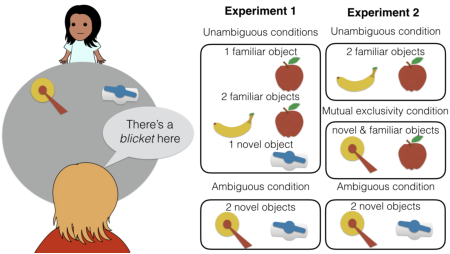
\includegraphics{figs/design-1} 

}

\caption[Study design for Experiments 1 and 2]{Study design for Experiments 1 and 2.}\label{fig:design}
\end{figure}
\end{CodeChunk}

\section{Experiment 1}\label{experiment-1}

In Experiment 1, we examined whether children would visually reference a
speaker more often when the speaker produced a referentially ambiguous
label compared to an unambiguous label. Children sat across from an
experimenter who labeled an object on the table between them (Figure
\ref{fig:design}). The experimenter then asked the child to place the
named object in a bucket. Across trials, there were either one or two
objects on the table, which were either familiar or novel to the child.
This design allowed us to test whether merely having more than one
object present is sufficient to increase social referencing (which could
not be ruled out by Vaish et al.), or if referential ambiguity (and thus
epistemic uncertainty) is the underlying factor. If the latter is true,
we expected children to increase their looking to the experimenter only
on trials with two unfamiliar objects, when the object-label mapping was
not known and could not be inferred.

We were interested in the amount of social referencing children
exhibited across the trial. We considered four different phases of each
trial based on the notion that children might expect different social
information at different stages of the task. Specifically, we predicted
that children might expect the speaker's gaze direction to be
informative during the labeling itself, as speakers tend to look at
objects they refer to. We predicted that later in the trial, as children
reached for an object and placed it in the bucket, they might expect
evaluative feedback about their choice (e.g., facial expressions of
encouragement or discouragement).

\subsection{Methods}\label{methods}

\subsubsection{Participants}\label{participants}

We recruited a planned sample of 80 children ages 2-5 years from the
Children's Discovery Museum in San Jose, California.\footnote{Planned
  sample size, exclusion criteria, and analysis plan preregistered at
  \url{https://osf.io/y7mvt}} The sample included 20 2-year-olds (mean
age 31.97 months), 20 3-year-olds (mean age 42.65 months), 20
4-year-olds (mean age 55.85 months), and 20 5-year-olds (mean age 65.21
months). An additional 20 children participated but were removed from
analyses because they heard English less than 75\% of the time at home
(\emph{n} = 10), because they were unable to complete at least half of
the trials in the task (\emph{n} = 4), because of parental interference
(\emph{n} = 1), or due to experimenter or technical errors (\emph{n} =
5).

\subsubsection{Stimuli and Design}\label{stimuli-and-design}

Children were presented with one or two objects, heard a label, and were
asked to put the labeled object in a bucket. Half of the objects were
selected to be familiar to children (e.g., a cow) and half were selected
to be novel (e.g., a nozzle). There were four trial types: one-familiar,
one-novel, two-familiar, and two-novel. There were three trials of each
type, for a total of twelve trials. Trial types were presented
sequentially in an order that was counterbalanced across participants.
The assignment of individual objects to trial types was counterbalanced.
On familiar trials, the familiar label for the target object was used
(e.g., ``cow''). On novel trials, a novel label was used (e.g.,
``dawnoo'').

The critical manipulation was of referential ambiguity; on one-familiar
and two-familiar trials, there was no referential ambiguity, as children
were expected to be certain about the objects and their labels.
Similarly, on one-novel trials, children were expected to be certain
about the label referent as there was only one option. However, on
two-novel trials, the referent was ambiguous, as the novel label could
apply to either novel object.

Throughout the task, the experimenter never gazed at the object they
were labeling, or responded to children's verbal or non-verbal bids for
help by indicating the correct object. Thus, children were expected to
remain uncertain about the referent throughout the trial when two novel
objects were present.

\subsubsection{Procedure}\label{procedure}

Throughout the study, the child sat at one end of a large circular
table, and the experimenter stood at the opposite end. Each trial of the
task proceeded as follows: the experimenter placed one or two objects on
the sides of the table, out of reach of the child so that the child
could not interact with the toys during the labeling event. For
one-object trials, the location of the object (left or right) alternated
between trials.

After placing the objects, the experimenter said ``Hey look, there's a
(target) here.'' The experimenter gazed at the center of the table
rather than the object they labeled (see rationale in Stimuli and
Design). The experimenter waited approximately two seconds (based on a
visual metronome placed within view) before saying, ``Can you put the
(target) in the bucket?'' They then pushed the object(s) forward within
reach of the child, and placed a plastic bucket in the center of the
table, also within reach of the child. Prior to the twelve experimental
trials, there were two training trials: a one-familiar trial and a
two-familiar trial, to acquaint the child with the procedure. A camera
placed to the side of the experimenter captured the participant's face,
so that looking behavior could be coded from video.

\subsubsection{Coding procedure}\label{coding-procedure}

Videos were coded using DataVyu software (\url{http://datavyu.org}). For
each participant, we coded the number of times they referenced the
experimenter across the trial. Because we were interested in the
circumstances that elicit social referencing in children, we coded the
number of looks that occurred during four phases of the trial: a
\emph{label} phase, which began at the utterance of the label and ended
when the experimenter began to slide the objects, a \emph{slide} phase,
in which the experimenter slid the object(s) into the child's reach, a
\emph{planning phase}, which began at the end of the slide and ended
when the child touched an object, and a \emph{response} phase, which
began when the child touched an object and ended when the child released
the object into the bucket. A second coder independently scored the
number of looks for one third of the trials for each participant to
establish reliability.

\subsection{Results and Discussion}\label{results-and-discussion}

\begin{CodeChunk}
\begin{figure*}[h]

{\centering 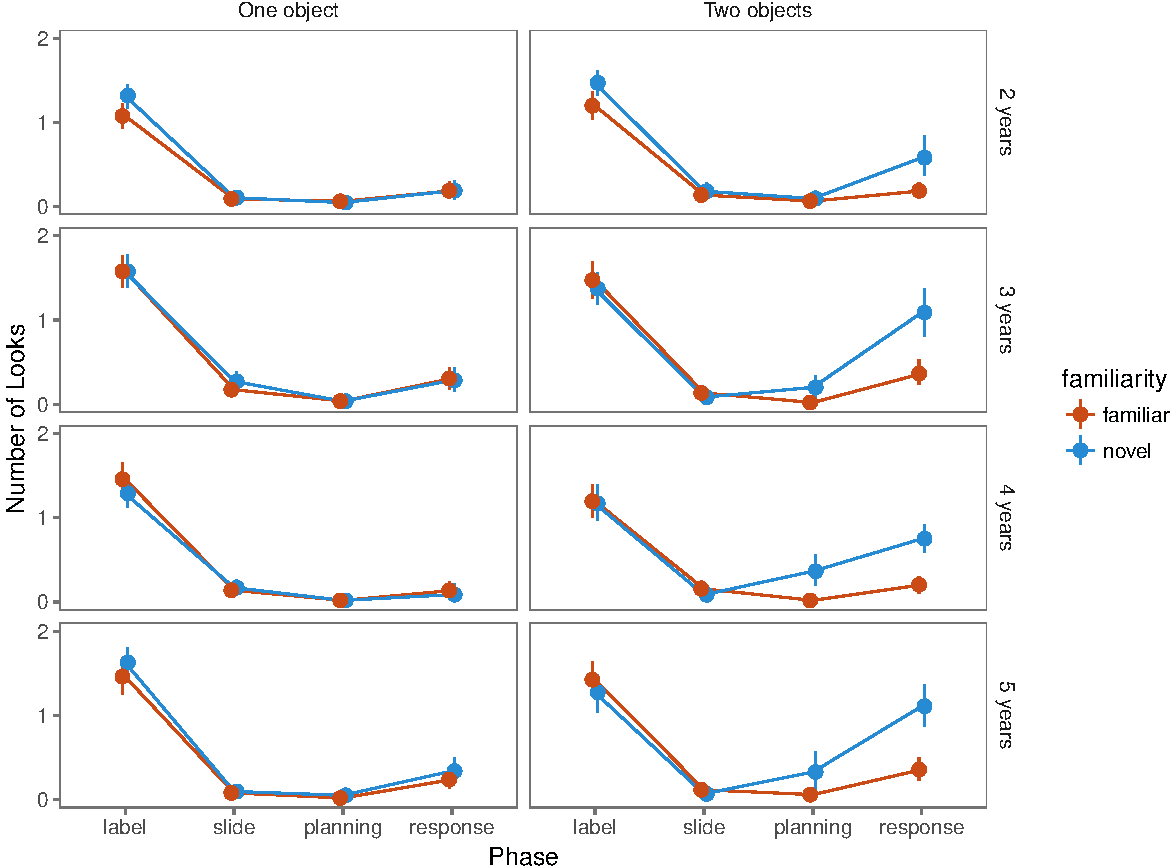
\includegraphics[width=5.75in,height=4.35in]{figs/results_e1-1} 

}

\caption[Results of Experiment 1]{Results of Experiment 1. Number of looks to the experimenter across phases and conditions. Error bars are 95 percent confidence intervals.}\label{fig:results_e1}
\end{figure*}
\end{CodeChunk}

Results of Experiment 1 are presented in Figure \ref{fig:results_e1}.
Inter-rater reliability for the number of looks in each phase was high,
intraclass correlation \emph{r} = .97, \emph{p}\textless{}.001. To test
our prediction that referential ambiguity (i.e., having two novel
objects) would produce more social referencing, we fit mixed-effects
linear regression models separately for each phase with the following
structure:
\texttt{number\ of\ looks\ \textasciitilde{}\ number\ of\ objects\ *\ familiarity\ *\ age\ in\ months\ +\ (number\ of\ objects\ +\ familiarity\ \textbar{}\ Subject\ ID)}.
A single model with phase as a factor did not converge.

We did not find any main or interaction effects of number of objects,
familiarity, or age on number of looks during the label or slide phases.
Thus, mere novelty or the presence of multiple objects was not enough to
increase social referencing. However, we found an interaction effect of
number of objects and familiarity during the planning (\emph{\(\beta\)}
= 0.21, \emph{p} \textless{} .001) and response phases (\emph{\(\beta\)}
= 0.6, \emph{p} \textless{} .001), such that 2-novel trials were
associated with more looking. There was no interaction with age in
either phase.\footnote{\url{https://github.com/emilyfae/socref_uncert}}
In summary, children looked to the experimenter more often when planning
and executing a response under uncertainty. These results suggest that
children were aware that they did not have sufficient knowledge to
answer independently, and referenced the speaker to resolve this
uncertainty.

We did not find the expected effect of referential ambiguity in the
label phase. It is possible that children failed to predict that they
would need more information until later in the trial, when they were
actually faced with making a decision. Another possibility is that
children's looking was at ceiling during the labeling phase, perhaps
because children look at someone who is speaking regardless of the need
for referential disambiguation. A third possibility is that this is an
artifact of our design, in which the experimenter gazed at the center of
the table rather than the referent of the label. Children may have
realized that the experimenter's gaze direction during labeling was not
informative. Similarly, children may have found it strange to interact
with an experimenter who did not gaze at the object they were labeling,
which may have produced unnatural patterns of social referencing.
Experiment 2 tests these possibilities and examines whether children's
social referencing is sensitive to graded uncertainty.

\section{Experiment 2}\label{experiment-2}

Experiment 2 was designed to replicate Experiment 1 and investigate
whether children's social referencing is sensitive to uncertainty based
on graded evidence about a label's referent. Since we did not observe
any difference between one-familiar and one-novel trials, we eliminated
single-object trials, leaving the 2-familiar and 2-novel trials. In
addition, we added 1-novel-1-familiar trials. For these trials, we
expected that children would be able to infer the referent by excluding
the familiar object as a possibility. For example, when a toy lion and a
novel item were present, they could exclude that the speaker was
referring to the lion as a ``blicket'' (Markman \& Wachtel, 1988). We
predicted that children might be less certain about their choice on
these trials compared to when the label and referent were familiar to
them (2-familiar trials), but more confident than when there are no cues
to reference (2-novel trials).

In addition, we manipulated between participants whether or not the
experimenter's gaze during labeling was informative (they gazed at
either the referent of their label or the center of the table), allowing
us to determine whether children selectively reference gaze during
labeling when gaze is expected to be informative. The manipulation of
informativity of gaze during labeling also meant that participants in
the referential gaze condition had an additional referential cue, which
might decrease uncertainty for the remainder of the trial. In Experiment
1, we did not observe an effect of age, so we restricted the current
sample to 3- and 4-year-olds.

\subsection{Methods}\label{methods-1}

\subsubsection{Participants}\label{participants-1}

We recruited a planned sample of 80 children ages 3-4 years from the
Children's Discovery Museum in San Jose, California.\footnote{Planned
  sample size, exclusion criteria, and analysis plan preregistered at
  \url{https://osf.io/y7mvt/}.}. The sample included 40 3-year-olds
(mean age 42.89 months) and 40 4-year-olds (mean age 53.47 months). An
additional 20 children participated but were removed from analyses
because they heard English less than 75\% of the time at home (\emph{n}
= 9), because they were unable to complete at least half of the trials
in the task (\emph{n} = 7), or due to experimenter or technical errors
(\emph{n} = 4).

\subsubsection{Stimuli and Design}\label{stimuli-and-design-1}

The stimuli and design were similar to Experiment 1, except that we
eliminated 1-object trials. Instead, we included three trial types:
2-familiar, 2-novel, and 1-novel-1-familiar. There were four of each
trial type, totaling twelve trials. In addition, we manipulated the
experimenter's gaze behavior between participants. For half of the
participants, the experimenter looked at the center of the table while
labeling objects; for the remaining half, they looked directly at the
objects they labeled.

\subsubsection{Procedure}\label{procedure-1}

The procedure was identical to Experiment 1, except that there were
three practice trials (two familiar trials and one novel trial). We
included two familiar trials during the practice so that children would
remain motivated to complete the task.

\subsection{Results and Discussion}\label{results-and-discussion-1}

\begin{CodeChunk}
\begin{figure*}[h]

{\centering 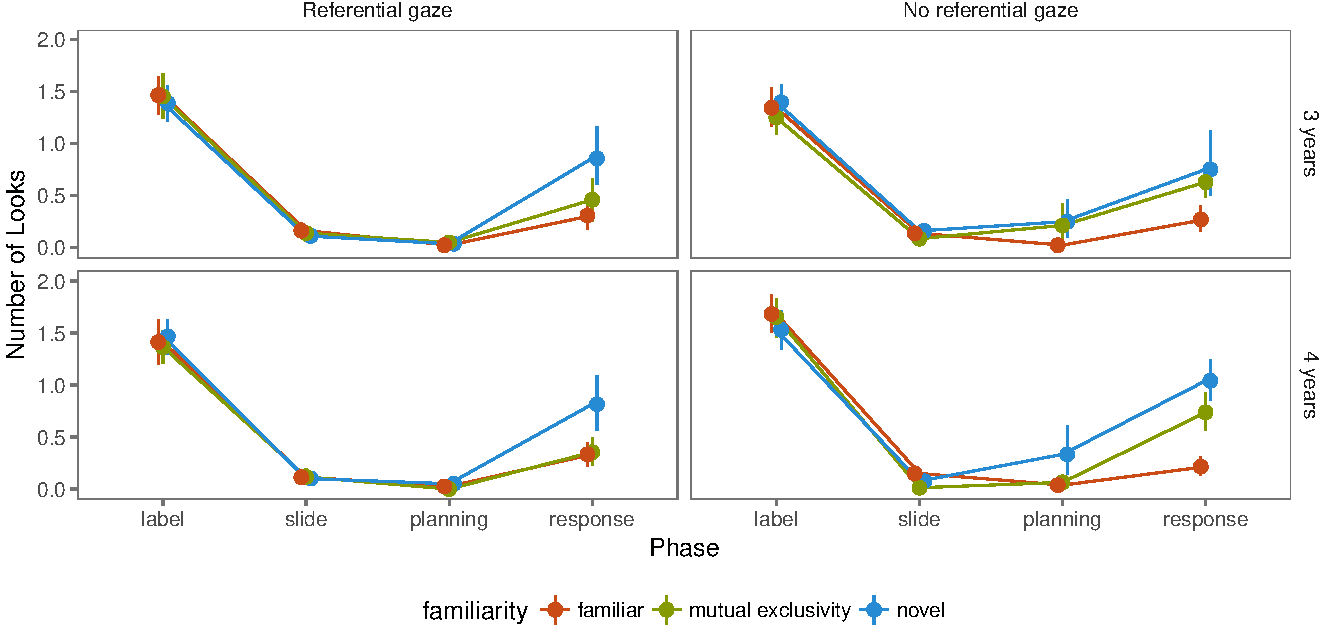
\includegraphics[width=5.75in,height=3.5in]{figs/results_e2-1} 

}

\caption[Results of Experiment 2]{Results of Experiment 2. Number of looks to the experimenter across phases and trial types. Error bars are 95 percent confidence intervals.}\label{fig:results_e2}
\end{figure*}
\end{CodeChunk}

Results of Experiment 2 are presented in Figure \ref{fig:results_e2}.
Inter-rater reliability for the number of looks in each phase was again
high, intraclass correlation \emph{r} = .97, \emph{p}\textless{}.001. To
quantify the main and interactive effects of familiarity, gaze
informativity, phase, and age on social referencing, we fit a
mixed-effects linear regression model with the following structure:
\texttt{number\ of\ looks\ \textasciitilde{}\ familiarity\ *\ age\ in\ months\ *\ gaze\ *\ phase\ +\ (familiarity\ \textbar{}\ Subject\ ID)}.
In contrast to Experiment 1, a model with phase as a predictor
converged.

First, do children reference a speaker more often when the objects and
label are novel? Phase interacted with familiarity such that the
response phase of novel trials was associated with significantly more
looks (\textbf{\(\beta\)} = 0.51, \emph{p} \textless{} .001). This
result is consistent with our finding from the analysis of the response
phase in Experiment 1. However, in contrast to Experiment 1, we did not
observe that looking was significantly greater for novel trials in the
planning phase.

We were also interested in whether mutual exclusivity trials would
elicit an intermediate amount of uncertainty. We observed a three-way
interaction of familiarity, gaze, and phase, such that the response
phase of mutual exclusivity trials in the no-referential-gaze condition
was associated with significantly more looks (\emph{\(\beta\)} = 0.39,
\emph{p} \textless{} .01). Thus, mutual exclusivity trials were
associated with greater looking only when the experimenter did not
provide informative gaze. This finding is intriguing given that children
should be able to solve mutual exclusivity trials without gaze
information. Instead, they appear to remain relatively uncertain while
making a decision if excluding the familiar object is their only cue to
reference, but this uncertainty is resolved if the speaker's gaze is
informative. On the other hand, informative gaze during labeling did not
lessen social referencing for novel trials, suggesting that gaze
information alone was not sufficient to reduce uncertainty. Instead,
both gaze information and mutual exclusivity provided evidence about a
label-object pairing, and children required both types of evidence to
feel certain about their response.

Finally, we observed a four-way interaction such that the response phase
of novel trials in the gaze condition was associated with more looking
with increasing age (\emph{\(\beta\)} = 0.06, \emph{p} \textless{} .01),
suggesting that children may become more selective in their social
referencing as they get older. It may be that children improve in their
ability to monitor the need for disambiguating information, or they may
become more likely to recognize that social information can be a source
of disambiguation.

We did not observe social referencing during the label phase, even when
referential gaze was available. This result rules out the possibility
that children were less selective during labeling because they learned
that gaze direction was not informative.

\section{General Discussion}\label{general-discussion}

During the preschool years, children are increasingly able to actively
gather information through help-seeking and exploration (Chouinard et
al., 2007; Schulz \& Bonawitz, 2007). Do children monitor their own
uncertainty to guide these behaviors, or are they indiscriminate with
regard to underlying knowledge states? Here, we examined whether young
children's social referencing during a word-learning task was driven by
uncertainty about a label's referent.

We found that referential ambiguity strongly predicted children's social
referencing. Specifically, we observed this selectivity when children
were forced to decide which object the speaker was referring to. We
speculate that children referenced the speaker during the decision
process because they expected evaluative feedback about their choice,
either implicitly through the adult's facial expressions, or through an
explicit response. This idea is consistent with other recent research
that has found that preschoolers seek help selectively when a problem is
difficult or they are less skilled (Vredenburgh \& Kushnir, 2015).

Most intriguingly, we found that children's looking was driven by graded
referential evidence. In the case of mutual exclusivity trials, children
could solve the problem of reference by excluding the familiar item
(Markman \& Wachtel, 1988). Thus, unlike novel trials, they likely had
some signal about the correct object-label mapping. If children simply
monitored the presence or absence of such signals, they would have
consistently treated mutual exclusivity trials as familiar trials.
Instead, their social referencing depended on a combination of cues from
mutual exclusivity and gaze informativity, suggesting that they are
sensitive to graded evidence and seek disambiguating information only
when uncertainty is relatively high. Children's greater social
referencing on trials with only one cue to reference (i.e., mutual
exclusivity trials with no referential gaze and novel trials with
referential gaze) additionally suggests that children may remain
uncertain about a new label-object mapping if they have not received
confirmation of its accuracy, for example, through explicit feedback or
gaze direction.

On the other hand, we found no evidence for selective social referencing
as the object was being labeled. One possibility is that young children
do not recognize the need for disambiguating information until they need
to make a decision. Another possibility is that preschool-aged children
spontaneously look at a speaker regardless of ambiguity, and additional
looking was not needed or possible. Notably, Vaish et al. observed
selective referencing during labeling among infants. Since infants in
that study were holding one of the objects during labeling, referencing
the speaker would have required them to disengage from that object, and
may therefore have been more costly, promoting selectivity. Future
research with preschoolers that includes a greater reward trade off
between attentional options would help to distinguish among these
possibilities. Overall, these results provide evidence that
preschool-aged children monitor graded uncertainty in their mental
representations and act on that uncertainty through spontaneous
information-seeking.

\section{Acknowledgements}\label{acknowledgements}

We thank Veronica Cristiano for assisting with data collection. This
work supported by a generous gift from Kinedu, Inc.

\section{References}\label{references}

\setlength{\parindent}{-0.1in} \setlength{\leftskip}{0.125in} \noindent

\hypertarget{refs}{}
\hypertarget{ref-Baldwin1991}{}
Baldwin, D. A. (1991). Infants' contribution to the achievement of joint
reference. \emph{Child Development}, \emph{62}(5), 875--890.

\hypertarget{ref-Call2001}{}
Call, J., \& Carpenter, M. (2001). Do apes and children know what they
have seen? \emph{Animal Cognition}, \emph{3}(4), 207--220.

\hypertarget{ref-Carpenter1998}{}
Carpenter, M., Nagel, K., Tomasello, M., Butterworth, G., \& Moore, C.
(1998). Social cognition, joint attention, and communicative competence
from 9 to 15 months of age. \emph{Monographs of the Society for Research
in Child Development}, \emph{63}(4), i--iii--v--vi--1--174.

\hypertarget{ref-Chouinard2007}{}
Chouinard, M. M., Harris, P. L., \& Maratsos, M. P. (2007). Children's
questions: A mechanism for cognitive development. \emph{Monographs of
the Society for Research in Child Development}, \emph{72}, 1--129.

\hypertarget{ref-Coughlin2015}{}
Coughlin, C., Hembacher, E., Lyons, K. E., \& Ghetti, S. (2015).
Introspection on uncertainty and judicious help-seeking during the
preschool years. \emph{Developmental Science}, \emph{18}(6), 957--971.

\hypertarget{ref-Csibra2006}{}
Csibra, G., \& Gergely, G. (2006). Social learning and social cognition:
The case for pedagogy. In Y. Munakata \& M. H. Johnson (Eds.),
\emph{Processes of change in brain and cognitive development} (pp.
249--274). Oxford: Oxford University Press: Oxford University Press.

\hypertarget{ref-Dunlosky2012}{}
Dunlosky, J., \& Rawson, K. A. (2012). Overconfidence produces
underachievement: Inaccurate self evaluations undermine students
learning and retention. \emph{Learning and Instruction}, \emph{22}(4),
271--280.

\hypertarget{ref-Goupil2016}{}
Goupil, L., Romand-Monnier, M., \& Kouider, S. (2016). Infants ask for
help when they know they don't know. \emph{Proceedings of the National
Academy of Sciences}, \emph{113}(13), 3492--3496.

\hypertarget{ref-Hembacher2014}{}
Hembacher, E., \& Ghetti, S. (2014). Don't look at my answer: Subjective
uncertainty underlies preschoolers' exclusion of their least accurate
memories. \emph{Psychological Science}, \emph{25}(9), 1--9.

\hypertarget{ref-Ho2017}{}
Ho, M. K., MacGlashan, J., Littman, M. L., \& Cushman, F. (2017). Social
is special: A normative framework for teaching with and learning from
evaluative feedback. \emph{Cognition}, 1--16.

\hypertarget{ref-Lipowski2013}{}
Lipowski, S. L., Merriman, W. E., \& Dunlosky, J. (2013). Preschoolers
can make highly accurate judgments of learning. \emph{Developmental
Psychology}, \emph{49}(8), 1505--1516.

\hypertarget{ref-Lyons2011}{}
Lyons, K. E., \& Zelazo, P. D. (2011). Monitoring, metacognition, and
executive function: Elucidating the role of self-reflection in the
development of self-regulation. \emph{Advances in Child Development and
Behavior}, \emph{40}, 379--412.

\hypertarget{ref-Markman1988}{}
Markman, E. M., \& Wachtel, G. F. (1988). Children's use of mutual
exclusivity to constrain the meanings of words. \emph{Cognitive
Psychology}, \emph{20}, 121--157.

\hypertarget{ref-Robinson1997}{}
Robinson, M. D., Johnson, J. T., \& Herndon, F. (1997). Reaction time
and assessments of cognitive effort as predictors of eyewitness memory
accuracy and confidence. \emph{Journal of Applied Psychology},
\emph{82}, 416--425.

\hypertarget{ref-Schulz2007}{}
Schulz, L. E., \& Bonawitz, E. B. (2007). Serious fun: Preschoolers
engage in more exploratory play when evidence is confounded.
\emph{Developmental Psychology}, \emph{43}(4), 1045--1050.

\hypertarget{ref-Sodian2012}{}
Sodian, B., Thoermer, C., Kristen, S., \& Perst, H. (2012).
Metacognition in infants and young children. In M. J. Beran, J. Brandl,
J. Perner, \& J. Proust (Eds.), \emph{Foundations of metacognition} (pp.
119--133).

\hypertarget{ref-Vaish2011}{}
Vaish, A., Demir, Ö. E., \& Baldwin, D. A. (2011). Thirteen- and
18-month-old infants recognize when they need referential information.
\emph{Social Development}, \emph{20}(3), 431--449.

\hypertarget{ref-Vredenburgh2015}{}
Vredenburgh, C., \& Kushnir, T. (2015). Young children's help-seeking as
active information gathering. \emph{Cognitive Science}, \emph{40}(3),
697--722.

\hypertarget{ref-Walden1988}{}
Walden, T. A., \& Ogan, T. A. (1988). The development of social
referencing. \emph{Child Development}, \emph{59}(5), 1230--1240.

\hypertarget{ref-Yurovsky2015}{}
Yurovsky, D., \& Frank, M. C. (2015). An integrative account of
constraints on cross-situational learning. \emph{Cognition},
\emph{145}(C), 53--62.

\end{document}
